\documentclass[12pt,fleqn]{article}\usepackage{../../common}
\begin{document}
Turevsiz Optimizasyon (Derivative-free Optimization)

\begin{minted}[fontsize=\footnotesize]{python}
from mpl_toolkits.mplot3d import Axes3D
from matplotlib import cm
\end{minted}


\begin{minted}[fontsize=\footnotesize]{python}
def Rosenbrock(x,y):
    return (1 + x)**2 + 100*(y - x**2)**2

x = np.linspace(-2,2,250)
y = np.linspace(-1,3,250)
X, Y = np.meshgrid(x, y)
Z = Rosenbrock(X, Y)

fig = plt.figure(figsize = (8,4))

ax = fig.add_subplot(1, 2, 1, projection='3d')
ax.plot_surface(X,Y,Z,rstride = 5, cstride = 5, cmap = 'jet', alpha = .4, edgecolor = 'none' )
ax.view_init(0, 100)
ax.set_xlabel('x')
ax.set_ylabel('y')

ax = fig.add_subplot(1, 2, 2, projection='3d')
ax.plot_surface(X,Y,Z,rstride = 5, cstride = 5, cmap = 'jet', alpha = .4, edgecolor = 'none' )
ax.view_init(40, 250)
ax.set_xlabel('x')
ax.set_ylabel('y')

plt.savefig('func_70_dfo_01.png')
\end{minted}

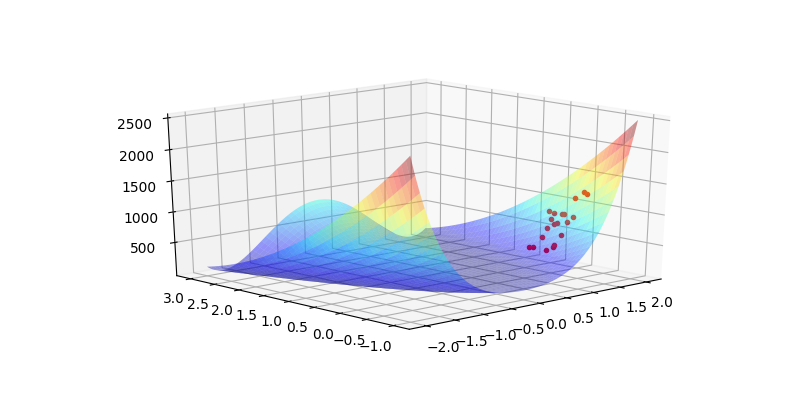
\includegraphics[width=35 em]{func_70_dfo_01.png}

\begin{minted}[fontsize=\footnotesize]{python}
def Peaks(x1,x2):
    return \
    3*(1-x1)**2 * np.exp(-x1**2 - (x2 + 1)**2) - \
    10*(1/5. * x1 - x1**3 - x2**5) * np.exp(-x1**2 - x2**2) - \
    1/3. * np.exp(-(x1+1)**2 - x1**2)

def Himmer(x,y):
    return (x**2 + y - 11)**2 + ( x + y**2 - 7 )**2

x = np.linspace(-3,3,100)
y = np.linspace(-3,3,100)
X, Y = np.meshgrid(x, y)
#Z = Himmer(X, Y)
Z = Peaks(X, Y)

fig = plt.figure()
ax = fig.gca(projection='3d')
ax.plot_surface(X,Y,Z, cmap=cm.jet, rstride=1, cstride=1)
ax.view_init(36, -124)
ax.set_xlabel('x')
ax.set_ylabel('y')

plt.savefig('func_70_dfo_02.png')
\end{minted}

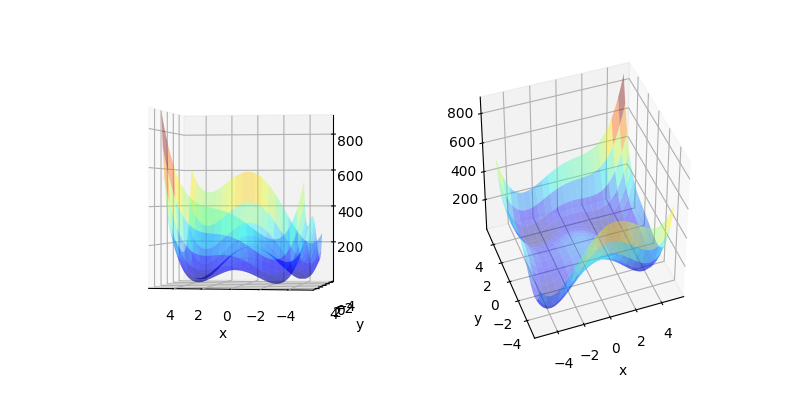
\includegraphics[width=35 em]{func_70_dfo_02.png}


kdkjflkajsdk lkj sdlfjalsjddlkslf


[devam edecek]

\end{document}
